\documentclass{standalone}
\usepackage{tikz}
\usepackage{tikz-qtree}
\usetikzlibrary{backgrounds, fit}

\begin{document}
  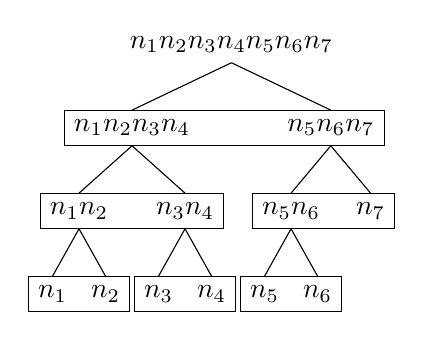
\begin{tikzpicture}
	\Tree [.\node (1234567) {$n_1n_2n_3n_4n_5n_6n_7$};
	  [.\node (1234) {$n_1n_2n_3n_4$};
		[.\node (12) {$n_1n_2$}; 
		  [.\node (1) {$n_1$}; ]
		  [.\node (2) {$n_2$}; ]] 
		[.\node (34) {$n_3n_4$};
		  [.\node (3) {$n_3$}; ]
		  [.\node (4) {$n_4$}; ]]] 
	  [.\node (567) {$n_5n_6n_7$};
		[.\node (56) {$n_5n_6$};
		  [.\node (5) {$n_5$}; ] 
		  [.\node (6) {$n_6$}; ]]
		[.\node (7) {$n_7$}; ]]]

	\begin{pgfonlayer}{background}
	  % \node () [ellipse, draw, fit = (1234567), inner sep = 0pt] {};

	  \node () [rectangle, draw, fit = (1) (2), inner sep = 0pt] {};
	  \node () [rectangle, draw, fit = (3) (4), inner sep = 0pt] {};
	  \node () [rectangle, draw, fit = (5) (6), inner sep = 0pt] {};
	  \node () [rectangle, draw, fit = (12) (34), inner sep = 0pt] {};
	  \node () [rectangle, draw, fit = (56) (7), inner sep = 0pt] {};
	  \node () [rectangle, draw, fit = (1234) (567), inner sep = 0pt] {};
	\end{pgfonlayer}
  \end{tikzpicture}
\end{document}
